\sectionlink{デコヒーレンスと量子計算}
% 原文 p.293
\hypertarget{srcpage:293}{}\label{srcpage:293}
量子情報理論と量子計算は、過去10年のあいだに急速に大きな関心を集め、理論的・実験的研究の焦点の一つになった。量子情報理論は、量子力学の多くの基本概念を、新しい視点から捉える。また、将来量子コンピューターを構築する可能性を含め、量子技術とその応用に関する提案を促してもきた。有用なアルゴリズムを実行する量子コンピューターは、実験的実現にはまだほど遠いが、多くの考えが検討され、量子コンピューターの基本的な構成要素となりうる部品のいくつかは、すでに実験室で開発されている。

同時に、量子情報理論と量子計算の研究は、デコヒーレンス効果の研究と制御への関心を飛躍的に高めた。基礎的な観点から見ると、環境とのvon Neumann型測定相互作用としてのデコヒーレンスの基本的な形式的記述（2.5.1節と2.6.3節参照）は、条件付き量子力学の形式を使って、量子情報理論の言葉で表し直せる\cite{ref016,ref323}（後の7.4.1節も参照）。さらに、本書の前の章でもすでに、デコヒーレンスと（かなり曖昧な）「情報」の概念との結び付きに触れた。具体的には、環境とのもつれが、どの状態にあるかという情報を運び去り、デコヒーレンスをもたらす仕組みの議論で、この結び付きを示した（2.6節参照）。実用的な観点からは、どのような量子コンピューターも、その動作は量子コヒーレンスを維持する能力に決定的に依存する。デコヒーレンスは計算に誤りを生じさせるため、量子コンピューターの実現にとって最大の障害である。

本章では、量子計算においてデコヒーレンスが果たす役割を概説する。7.1節では、量子計算と古典計算の主要な違い、および量子計算の基礎にある中心的な考えの歴史的発展を含め、量子計算の基本的側面を振り返る。7.2節では、量子コンピューターのどのような実現でも核心となる、デコヒーレンスと制御可能性のあいだのトレードオフを論じる。続く7.3節では、量子計算という主題に即して、デコヒーレンスと雑音の違いについて、さらにいくつか述べる（2.12節も参照）。7.4節では、いわゆる量子誤り訂正によって、量子コンピューターで有害なデコヒーレンスの影響を軽減する方法を説明する。
% 原文 p.294
\hypertarget{srcpage:294}{}\label{srcpage:294}
最後に7.5節では、2.8.1節で導入したデコヒーレンスのない（すなわちポインター）部分空間の概念を用いる量子計算を論じる。量子情報理論と量子計算全般についてさらに学びたい読者は、たとえばNielsenとChuangの著書\cite{ref056}に多くの内容を見いだすだろう。

\subsectionlink{量子計算の概観}
今日買ったコンピューターが、ほんの数年後には救いようもなく時代遅れになることは、誰もが知っている。過去数十年間にコンピューターが高速化した速さは、驚異的としかいいようがない。それに伴い、コンピューターのプロセッサーを構成する回路の複雑さ（たとえば、チップ当たりのトランジスター数で測る）は、急速に増え続けている。読者は、回路の複雑さがおよそ2年ごとに倍になるという、Mooreの有名な「法則」を聞いたことがあるかもしれない。この予測は、これまで驚くほど正確であった。

この結果、1970年代と1980年代の少数の研究者たちは、ある時点でチップ上の個々の処理構造（たとえばトランジスター）が、量子効果が重要になる原子スケールに達するはずだと気付いた。\footnote{Moore自身は1997年の講演で、これが2017年ごろに起こると予測した\cite{ref324}。}そこから、こうした量子効果を実際に利用して計算能力を高められるのか、という考察へ導かれた。さらに大胆にいえば、量子力学の原理を巧みに使うことに、その能力が特に依存するようなコンピューターを作れるだろうか。

\subsubsectionlink{量子計算の能力}
本質的に量子的なコンピューターが、なぜ通常の（「古典的な」）コンピューターよりはるかに強力になりうるのか、少し考えてみよう。古典コンピューターは、論理ビットという基本単位で情報を符号化する。その値は「0」か「1」のいずれかを取る。量子情報理論の主要な標語は、「情報は必然的に物理的である」というものである（この洞察をおそらく最初に強調したのはLandauer\cite{ref325}であった）。紙上の鉛筆の線であれ、トランジスター中の電子の存在であれ、情報はつねに何らかの物理系によって符号化されなければならない。したがって、情報の符号化自体が物理法則に従う。

そこで、ビット値「0」と「1」に対応する二状態を取りえ、そのため1ビットの情報を符号化できる物理系を考えよう。コンピューターの構成要素が小さくなるという先の議論に沿えば、この系は、古典的に区別可能で、古典ビットの二つの値に対応する二つの基底状態$|0\rangle$と$|1\rangle$をもつ量子系であってよい。
% 原文 p.295
\hypertarget{srcpage:295}{}\label{srcpage:295}
このような「量子ビット」の系は、2.10節と第5章ですでに論じた。原理的には、実効的に二次元の状態空間をもつ任意の量子系を量子ビットとして用いられる。その例は、二つの偏光自由度をもつ光子、イオンや原子核のスピン、および二つの支配的なエネルギー準位をもつ原子である。これらの物理的実現のいくつかは、後の7.1.5節で説明する。

量子力学によれば、この系は、少なくとも原理的には（すなわち$\{|0\rangle,|1\rangle\}$基底でのデコヒーレンスを無視できれば）、コヒーレントな重ね合わせ
\begin{equation}|\psi\rangle=\alpha|0\rangle+\beta|1\rangle\tag{7.1}\end{equation}
にもなりうる。大ざっぱにいえば、値が0か1のいずれかである古典ビットとは異なり、量子ビットは二つの論理ビット0と1を同時に符号化できることを意味する。係数$\alpha$と$\beta$の選び方は無限にあるため、一つの量子ビットが取りうる状態は、古典ビットの二状態に対して無限に存在する。与えられた状態$|\psi\rangle$にある一つの量子ビットは、二つの実数を符号化できるが、古典ビットは一つの2進数字しか表さない。これは、$|\psi\rangle$がつねに
\begin{equation}|\psi\rangle=|\alpha|e^{i\phi_0}|0\rangle+|\beta|e^{i\phi_1}|1\rangle\tag{7.2}\end{equation}
と書けることからわかる。物理的に関係のない全体の位相因子を無視すれば、これは
\begin{equation}|\psi\rangle=|\alpha||0\rangle+|\beta|e^{i(\phi_1-\phi_0)}|1\rangle\tag{7.3}\end{equation}
と表される。規格化条件$|\langle\psi|\psi\rangle|^2=1$を用いると、さらに
\begin{equation}|\psi\rangle=\cos\left(\frac{\theta}{2}\right)|0\rangle+\sin\left(\frac{\theta}{2}\right)e^{i\phi}|1\rangle\tag{7.4}\end{equation}
と書き直せる。ここで$\phi\equiv\phi_1-\phi_0$であり、角$\theta$を適切に選ぶ（$0\leq\theta\leq\pi$）。式(7.4)は、このような状態をBloch球の描像によって見やすく可視化できる形である（図7.1参照）。こうして、無限に存在する単一量子ビット状態のどれも、二つの実数（ここでは角$\theta$と$\phi$）を符号化することを示した。

今度は、系が$N$個の量子ビットから構成されるとしよう。この系のHilbert空間は、単一量子ビットのHilbert空間$\mathcal H_i$（$1\leq i\leq N$）のテンソル積$\mathcal H=\mathcal H_1\otimes\mathcal H_2\otimes\cdots\otimes\mathcal H_N$で与えられるため、次元は$2^N$である。したがって、互いに直交する$2^N$個の基底状態が存在する。通常、これらは第$i$量子ビット（$1\leq i\leq N$）の元の単一量子ビット基底状態$|0\rangle_i$と$|1\rangle_i$の積状態に選ばれる。
\begin{equation}\begin{aligned}|00\cdots0\rangle&\equiv|0\rangle_1|0\rangle_2\cdots|0\rangle_N,\\|00\cdots1\rangle&\equiv|0\rangle_1|0\rangle_2\cdots|1\rangle_N,\\&\ \vdots\\|11\cdots1\rangle&\equiv|1\rangle_1|1\rangle_2\cdots|1\rangle_N.\end{aligned}\tag{7.5}\end{equation}
% 原文 p.296
\hypertarget{srcpage:296}{}\label{srcpage:296}
\begin{figure}[htbp]\centering
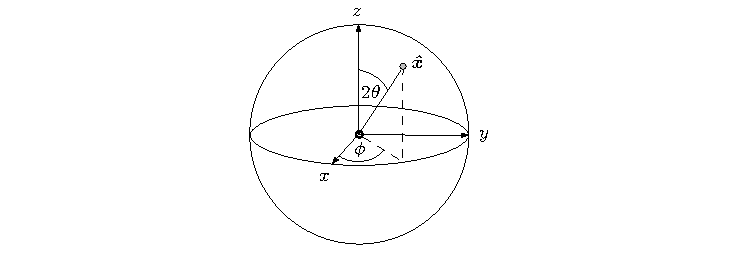
\includegraphics[width=.42\linewidth]{figures/ch07_fig01.pdf}
\caption{量子ビットの状態を、$\mathbb R^3$内の単位球であるBloch球上の点として幾何学的に表したもの。任意の量子ビット状態は二つの実パラメーター$\theta$と$\phi$で記述できる［式(7.4)参照］。ここで$2\theta$と$\phi$は、よく知られた球座標の役割を果たす。すなわち、状態(7.4)は単位ベクトル$\hat{\bm x}=(\sin2\theta\cos\phi,\sin2\theta\sin\phi,\cos2\theta)$によって表される。}
\end{figure}
この基底を、$N$量子ビット系の計算基底と呼ぶ。任意の$N$量子ビット状態は、$2^N\times2^N$の密度行列でも記述できる。この行列を対角化すれば、対角成分には$2^N$個の実数値（密度演算子の固有基底における占有数を表す）があるため、この状態は$2^N$個の独立な実数を同時に符号化できることがわかる。これに対して、$N$個の古典ビットが符号化するのは、長さ$N$の2進文字列にすぎない。ここに量子コンピューターの第一の利点がある。量子ビットの配列の記憶容量は古典ビットの配列より指数関数的に大きく、一つの量子ビットは、無限に存在するコヒーレントな重ね合わせ状態(7.1)のどれにもなれる。

第二の利点は、古典コンピューターと量子コンピューターが情報を処理する仕方の違いに関係する。古典コンピューターでは、一度に一つか二つのビットに作用する論理ゲート（AND、NOT、XORなど）を適用する。量子の場合、ゲートの実行は、$N$量子ビット系のHilbert空間に作用するユニタリー変換$\hat U$の適用に対応する。\footnote{量子計算には別の方法もあり、初めに高度にもつれた状態（いわゆるクラスター状態）へ準備した量子ビット系に対する、時間順に並んだ射影測定の列として、計算全体を進める\cite{ref326,ref327,ref328}。このような測定に基づく（またはクラスター状態）量子計算は、ユニタリーなゲート操作に基づく従来の量子計算と、まったく同じ計算課題を実行できることが示せる。言い換えれば、測定に基づく量子コンピューターは、「標準的な」量子コンピューターと同じく普遍的である。量子測定の非ユニタリー性からは、任意の（したがってユニタリーなものも含む）量子力学的時間発展のシミュレーションとは両立しないと直観的に考えそうであるため、これは注目すべき結果である。クラスター状態量子計算は、高度にもつれた$N$量子ビット状態を準備し、それを時間とともに生じるデコヒーレンスに対して十分頑健に保つ必要があるため、一般的なデコヒーレンスの性質は、ゲートに基づく量子計算と似ていると予想される。クラスター状態量子計算のわかりやすい入門として、文献\cite{ref329}を参照されたい。}

% 原文 p.297
\hypertarget{srcpage:297}{}\label{srcpage:297}
ここで鍵になるのは、このような変換$\hat U$は、一つの量子ビットにしか作用しない場合でも、$N$量子ビット系の大域的状態を変えうることである。たとえば最大にもつれた状態では、一つの量子ビットに加えたユニタリー操作が、一般に、全$N$量子ビットの大域的状態を変える。したがって、その操作は、全量子ビット系の$2^N$個の基底状態すべてに同時に作用する。簡単な例として、Bell型(2.7a)の二量子ビットもつれ状態
\begin{equation}|\Phi^+\rangle=\frac{1}{\sqrt2}(|00\rangle+|11\rangle)\tag{7.6}\end{equation}
に、第一の量子ビットだけに作用するユニタリー変換$\hat U$、たとえば
\begin{equation}\hat U=(-|0\rangle\langle1|+|1\rangle\langle0|)_1\otimes\hat I_2\tag{7.7}\end{equation}
を施すとしよう。変換後の状態は
\begin{equation}\hat U|\Phi^+\rangle=\frac{1}{\sqrt2}(|10\rangle-|01\rangle)\tag{7.8}\end{equation}
となる。この特徴は、もつれた多粒子状態の、非局所的で全体論的な性質の帰結と見ることができる。ここでも、古典的な状況と対比される。古典的には同じ操作を$2^N$回行うか、一つの古典論理ゲートをそれぞれ適用する$2^N$個の「プロセッサー」を並列に働かせる必要がある。\footnote{この観察との類推で、量子コンピューターは大規模な「量子並列性」を示すとよくいわれる（この特徴は、Zurekが早い時期に「量子Monte Carlo」の名で指摘した\cite{ref330}）。ただし、この用語は慎重に解釈すべきである。並列性は、多くの独立した過程が並列に実行されるという印象を与えるが、量子の場合には実際には、一つの量子力学的な「全体」（すなわち大域的な量子状態）が、一つの操作（量子ゲート）を受けると考えるべきである。}実際には、一度に一つか二つの量子ビットに作用する量子ゲートだけを考えればよい。一量子ビットゲートと二量子ビットゲートの、ある特定の集合が、任意の量子計算を実行するのに十分であることを示せるからである\cite{ref056,ref331,ref332,ref333,ref334}。多量子ビットゲートを物理的に実現するために必要な、三つ以上の量子ビットのあいだの相互作用を作り出すことは、実際には難しいので、これは非常に有用な結果である。

\subsubsectionlink{量子コンピューターの読み出し}
古典コンピューターでは、全ビットの最終値を単に読み出すだけで、計算結果を得る。これは、コンピューターの状態を変えることなく、いつでも行える。
% 原文 p.298
\hypertarget{srcpage:298}{}\label{srcpage:298}
量子計算で対応する手続きは、計算の最後に、いくつかの（あるいはすべての）量子ビットについて、選んだ基底で射影測定を行うことである。量子測定の標準理論によれば、これは$N$量子ビット系の大域的状態を、測定する基底の一状態へ収縮させ、個々に測定された各量子ビットと他の量子ビットのあいだに存在するもつれを破壊する。古典的な場合との主要な違いは、量子力学の測定が確率的であるという事実に関係する。すなわち、同一に準備した$N$量子ビット系の集まりに同じ量子ゲート列を適用しても、測定結果は一般に系ごとに異なる。指定できるのは、測定の際に系がある状態として見いだされる確率だけである（2.1節参照）。

同一の量子計算を繰り返した最後に、一般には単一の一貫した結果を得られないため、この事実は量子計算を本質的に無用なものにするように見えるかもしれない。したがって量子コンピューターは通常、少なくとも場合によっては、計算課題に正しい答えを与えない。しかし幸い、多くの状況では、ある出力が本当に正しい結果かどうかを確認するのは比較的容易である。たとえば、量子コンピューター上で整数を因数分解する有名なアルゴリズム（後の7.1.4節参照）は、つねに正しい答えを与えるわけではない。しかし、整数を素数に分解した結果が正しいかどうかは簡単に確認できるので、量子コンピューターの誤った結果は、単に人の手で捨てればよい。最終的に測定された状態が正しい解に対応する確率が十分に高ければ（たとえば、正解を得るために必要な実行回数が問題の大きさとともに指数関数的に増えなければ）、それでも量子コンピューターの能力を有利に利用したことになる。

\subsubsectionlink{物理系のシミュレーション}
ここで次の問いを考えよう。古典コンピューターは、少なくとも原理的には、量子系をつねにシミュレートできるだろうか。\footnote{自明なことを述べる恐れはあるが、量子コンピューターも任意の古典コンピューターをシミュレートできることを指摘しておく。そのためには、各量子ビットがどの時刻にも$|0\rangle$か$|1\rangle$のいずれかで記述され、それらの重ね合わせにはならないように、状態を準備して量子ゲートを適用すればよい。この点は、量子計算におけるデコヒーレンスの役割についての後の議論に直接関係する。デコヒーレンスは、$N$量子ビット系の計算基底状態(7.5)のコヒーレントな重ね合わせを破壊する傾向があり、そのため量子ビットを実効的に古典論理ビットのレジスターへと変える。すると量子コンピューターは「量子的な能力」を失う。古典コンピューターと同じ機能は実行できるが、それ以上のことはできなくなる。}たとえば、$N$量子ビット系の量子状態を$2^N\times2^N$の行列で表し、ゲート操作を表す別の$2^N\times2^N$行列を適用することで、その時間発展を模倣できると考えるかもしれない。しかし、注意すべき点が二つある。
% 原文 p.299
\hypertarget{srcpage:299}{}\label{srcpage:299}
第一に、すでに見たように、この方法は$N$が大きくなると、計算量が手に負えなくなる。行列の大きさと行列演算の回数（したがって記憶容量と処理能力への要求）が、$N$の増加とともに指数関数的に膨れ上がるためである。そのため、大きな量子系（言い換えれば、量子アルゴリズム）を古典コンピューターでシミュレートするのは、あらゆる実用上の目的に対して不可能になる。第二に、より基礎的な観点からは、Bellの定理\cite{ref030}によって、相関がBell不等式を破るような、離れた二つの相関した系を準備できる古典的機構は存在しないことが示される。したがって、このような（EPR/Bell型の）相関は、量子世界と量子計算に特有の特徴である\cite{ref335,ref336}。

量子系をどう効率よくシミュレートするかという問題は、量子計算研究の根源にある。Feynman\cite{ref335}は1982年の重要な論文で、自然界の他の任意の（量子）系の物理的振る舞いを効率よく模倣できる量子系を構築する問題を考察した。量子コンピューターも必然的に物理系でなければならないので、そのような系は普遍的な模倣装置であるだけでなく、普遍量子コンピューターでもある。Feynmanは、この普遍的な模倣装置を、最近接相互作用をもつスピンの格子によって模型化した。よく知られるように、彼は、この模型が原理的には、有限次元のHilbert空間で記述できる他の任意の量子系をシミュレートできることを示した。これは基礎的に重要な、真に画期的な発見であった。しかし、Feynmanの模型にはまだ欠点があった。新しい計算課題ごとに、一般にはスピン間相互作用の形と強さを変える必要があったのである。この要求を実際に実現するのは明らかに難しく、Feynmanは、支配するHamiltonianを利用者が自由に選ぶための物理的機構を指定しなかった。

したがって次の段階は、固定されたHamiltonian（すなわち特定の物理的構成）に基づき、量子コンピューターに施す操作を変えるだけで、任意の問題を解ける普遍量子コンピューターを考案することであった。これは、David Deutschが1985年の重要な論文\cite{ref337}で達成した。Deutschは、二状態系の集まりに基づく模型を使った。これらの系を合わせた状態に、ユニタリー変換の小さな集合（先に述べた「量子ゲート」）を適用すると、原理的には任意のユニタリーな時間発展を実現し、したがって任意の物理系をシミュレートできることを示した。可能な時間発展の広い一群に対しては、この量子コンピューターは効率よくも動作する\cite{ref338}。すなわち、ある時間発展を実現するのに必要な計算手順の数は、入力の大きさ（Deutschの模型では二状態系の数）に対して、指数関数より遅く増える。他の（ほとんど）どの物理系も効率よくシミュレートできることにより、Deutschの提案は、（ほとんど）普遍的な量子コンピューターの最初の設計図となった。

% 原文 p.300
\hypertarget{srcpage:300}{}\label{srcpage:300}
\subsubsectionlink{有名な量子アルゴリズムの例}
Deutschの論文に続く数年間、研究者たちは、古典コンピューターに対する量子コンピューターの優位性を示す計算課題を探すことに忙しかった\cite{ref339,ref340,ref341,ref342,ref343}。初期の試みはあまり実りがなかったが、1994年にPeter Shor\cite{ref344,ref345}が、因数分解問題（与えられた整数を素数の積へ分解する課題）を、多項式時間だけで解ける量子アルゴリズムを提示した。具体的には、$N$桁の数に対して$O(N^2)$の時間である。これに対して、古典コンピューターで因数分解問題を解くには、指数時間が必要だと広く考えられている（厳密に証明されてはいない）。したがって、相当に大きな数については、古典コンピューターでこの課題を達成するのは、本質的に不可能である。Shorの発見の重要性は、潜在的な実用的応用よりもむしろ、そのアルゴリズムが、Steane\cite{ref336}の言葉でいう「量子力学の本質の何かを定義するうえで、Bell不等式と同様の概念的役割」を果たすという点にあるのかもしれない。

量子計算分野を取り巻く初期から現在までの関心の多くは、Shorのアルゴリズムを根源とするといってよい。それ以来、量子コンピューターの能力を示す新しいアルゴリズムの発見は、比較的ゆっくりと進んできた（文献\cite{ref339,ref342}参照）。Shorのアルゴリズム以後で、おそらく最も重要な発見は、Groverの探索アルゴリズムである\cite{ref346,ref347}。このアルゴリズムは、非常に効率のよいデータベース探索を可能にする。構造をまったくもたない$N$項目のリストから、ある特定の項目を$O(\sqrt N)$の手順で見つけられる。これに対して、古典コンピューターでは、特定の項目を見つけるために、平均してリストの半分を調べる（すなわち$N/2$回の手順を行う）必要があるため、この課題には$N$程度の手順を要する。したがって、Groverのアルゴリズムを実行する量子コンピューターは、どのような古典コンピューターよりも$O(\sqrt N)$倍速い。

\subsubsectionlink{量子コンピューターの物理的実現}
上の量子計算への導入は、意図的にかなり抽象的なものにとどめた。ユニタリー変換（ゲート）の適用によってコヒーレントに操作できる、量子ビットの集まりが手元にあると、単に仮定しただけである。量子ビットの物理的性質も、こうしたゲート操作を実際にどう実行するかも指定しなかった。実際、量子コンピューターの原型（コヒーレントに制御できる、少数の量子ビットを含む系）の実験的実現に関する研究領域は広大であり、この急速に進む分野を概観しようとすることは、本書の範囲を完全に超える。

読者が最初の見当を得るために、表7.1では、将来、本格的な量子コンピューターへ発展する可能性のある、量子ビットと制御機構（ゲートと測定を実現する）の物理的実現の例をいくつか挙げる。各技術には長所と短所があり、それらは一般に、次の7.2節で論じる、デコヒーレンスと制御可能性のあいだの基本的なトレードオフに帰着する。
% 原文 p.301
\hypertarget{srcpage:301}{}\label{srcpage:301}
\begin{table}[htbp]\centering\small
\caption{量子ビット系と量子ビット制御の物理的実現の例。}
\begin{tabular}{lll}\hline
方式&量子ビットの実現&量子ビットの制御\\\hline
光学&光子&光学媒質\\
イオントラップ&捕獲イオン&レーザー光\\
共振器QED&二準位原子&レーザー光\\
NMR&核スピン&磁場\\
固体&結合した量子ドット&点接触\\
&超伝導トンネル接合&接合のバイアス電流\\\hline
\end{tabular}\end{table}
表7.1の構成要素を用いる現在の実験では、少数の量子ビットしかコヒーレントに制御できていない。有用な量子アルゴリズムを実行するには、はるかに多くの量子ビットが必要であり、したがって、これらの実験は量子コンピューターの実用的実現から、なお大きく隔たっている。
